%%
% This file is a sample of the main body of a dissertation
% at the Graduate School of Systems and Information Engineering,
% University of Tsukuba.
% You can rewrite this file to make a thesis body
% with the same format as this example using LaTeX.
% Depending on your PC environment and
% the settings of your LaTeX environment,
% you may need to change the kanji code and line feed code.
%%

\documentclass[12pt, a4paper]{report}
%\usepackage[utf8]{inputenc}

% IMPORTANT
\usepackage{sie-en}

\usepackage{graphicx} 
\usepackage{times}
\usepackage{xurl}

\usepackage{listings}
\usepackage{xcolor}
\usepackage{xltabular}
\usepackage{pdflscape}
\usepackage{afterpage}
\usepackage{float}
\usepackage{diagbox}
\usepackage{booktabs}
\usepackage[
    backend=biber,
    style=ieee,
  ]{biblatex}

\addbibresource{sample.bib}

\definecolor{dkgreen}{rgb}{0,0.6,0}
\definecolor{gray}{rgb}{0.5,0.5,0.5}
\definecolor{mauve}{rgb}{0.58,0,0.82}

\lstset{frame=tb,
  language=C++,
  aboveskip=3mm,
  belowskip=3mm,
  showstringspaces=false,
  columns=flexible,
  basicstyle={\small\ttfamily},
  numbers=none,
  numberstyle=\tiny\color{gray},
  keywordstyle=\color{blue},
  commentstyle=\color{dkgreen},
  stringstyle=\color{mauve},
  breaklines=true,
  breakatwhitespace=true,
  tabsize=3
}

\setcounter{tocdepth}{3}
\setcounter{page}{-1}

\title{Walking Aid Usage Prompt System}

\author{Sean Coaker, Pedro Caetano, \\Panayiotis Melios, Matthew Culley}

\programfield{CSCM04 Milestone 2}

\advisor{Tom Owen}

%% Name of department + year and month
%% Please rewrite as necessary.
\majorfield{MEng Computing}

\graduateyear{2022}
\graduatemonth{March}

\abstract{
    \noindent
    
}
%%%%%

\begin{document}

\maketitle
\makeabstract
\maketableofcontents

%\pagenumbering{roman} % I, II, III, IV {}
%{
%  \setlength{\parskip}{0pt}
%  \tableofcontents
%  \listoffigures
%  \listoftables
%}
%\pagebreak \setcounter{page}{1}
%\pagenumbering{arabic} % 1,2,3

\chapter{Introduction}

The opportunity of developing the walking aid usage prompt system emerged when Bangor Health Clinic reached out to us in need of a solution that helps remind dementia patients to use their walking aids when walking. Since that initial meeting, we developed a bi-device system that detects when the patient is walking without their walking aid and plays an audio reminder to the patient, or a vibration reminder through a wearable device if the patient is hearing deficient. 

The bi-device system encompasses a device to be attached to the patient's walking aid and another device to be attached to the patient. Utilising the monitoring of changes in gravity through accelerometers, we have created a system that can detect when the patient has started walking, and whether the walking aid is moving also. We implemented an algorithm that signifies that the patient is walking when the accelerometer detects that they have made 5 steps in the space of a 10 second period. Communication is then made to the walking aid device, which runs a check to see if it has been moved in the last 10 seconds, or is moved in the next 10 seconds. If neither occurs, either an audio reminder is played to the user, or the wearable device receives a message back from the walking aid device asking it to vibrate for patients who are hard of hearing. 

The following document consists of a design section, where we will detail the design decisions we made for each device, and acceptance testing section, which will contain evidence that the system was tested to ensure full functionality, and a narrative and reflective account section, where we will provide a narrative account of the process of developing the project and a reflection on what we could have done better had we avoided mistakes and been offered more resources to complete the project.
\chapter{Current Progress}

Within this chapter we will detail the progress we have made towards completing the product set out to be developed within this project. This chapter will consist of a section detailing what work was carried out prior to the submission of our milestone 1 document on December 14th, and what work has been carried out since then. We will also detail any issues that we have faced along the way that may have hampered the progress we wanted to make and may have impacted upon the schedule we detailed in our milestone 1 document.

\section{Progress Prior to Milestone 1}

Prior to the submission of our milestone 1 document, we had held 2 meetings with our client to gain an understanding of the user requirements for the project and to clarify details within project management such as the budget we were assigned and if the client had any preferences towards what hardware we should use to develop our product.

We held an introductory meeting with the client on the 18th of November, which allowed us to clarify what issue the client wanted to solve and what system the client desired to be built to solve said issue. Unfortunately, we left the meeting feeling unsatisfied as we had failed to gain a full understanding of the final direction the client wanted the project to go down. We were left with two options; to develop a non-wearable device, such as a pressure pad system, to detect when the patient had left their resting area, or to develop a wearable device that would constantly poll an accelerometer to detect the patient walking. The client kindly agreed to offer us a budget of £150 to aid with the procurement of hardware devices that were a necessity for developing the product depending on the route we decided to take the project down.

Due to the fact that we had left the introductory meeting without a clear set of final user requirements, we held an intra-team meeting to decide upon which solution we would prefer to develop as a team, both based on the skills we posses in code development and engineering, as well as what we felt would be most beneficial to solving the problem at hand. We ultimately decided to develop a product that included the wearable device. We decided on this solution as we felt that it offered the best platform to incorporate stretch features, such as fall detection in future. It also avoids some clear disadvantages from using a pressure pad system such as a carer needing to move the pressure pad to each piece of furniture the patient rests on, and creating a water proof solution that means that the pressure pad can be easily cleaned.

Once we had clarified the route we wanted to take the project down, we scheduled a second meeting with the client for the 25th of November to discuss our decision with them. The client agreed with our reasoning for developing a wearable device and were content for the project to continue in this manner. We finalised a final budget of £150 and the client stated that they did not have any preference for hardware to be used within the development of this system. We agreed with the client that we would develop a list of functional and non-functional requirements for them to agree to or amend where they saw fit, and would include them within the submission of our milestone 1 document. Our next steps from here were to complete the milestone 1 document, and finalise a list of hardware devices that were necessary for the development of the system we had in mind. Once we had finalised a list of hardware devices to procure, we needed to submit them to the client for ordering so that we could begin code development.

\section{Progress Since Milestone 1}

Within this section we will detail the work that we have carried out since the submission of our milestone 1 document. This will include an insight into the challenges we faced in procuring the hardware needed for this project, research that was made into relative code that can be used to detect to walking or to provide communication between our devices, before finally discussing the code we have developed so far along with insights into the challenges we faced with the code and how we overcame them. Each challenge stated will have accompanying discussion as to how they may or may not have negatively affected our project progress both in terms of schedule and/or financing.

\subsection{Hardware Procurement}

The hardware procurement task of the project required our team to come together to agree upon a platform to develop our code on, as well as any additional devices that needed to be connected in order to allow us to meet the client's specified requirements. Our team unanimously voted to work on the Arduino platform, as it offers extensive hardware and documentation options, as well as the option to develop code in either of the Arduino C programming language or MicroPython. Once we had all agreed which platform to develop code on, we set about finalising a list of hardware devices to order. A table of the devices we intended to order, their worst case unit price, quantity, worst case total price and a description of their involvement within this project can be seen on the next page in table \ref{tbl:items}.

\afterpage{%
    \clearpage% Flush earlier floats (otherwise order might not be correct)
    \thispagestyle{empty}% empty page style (?)
    \begin{landscape}% Landscape page
        \centering % Center table
        \small
		\begin{xltabular}[H]{1.4\textwidth}{p{0.15\textwidth} | p{0.15\textwidth} | p{0.15\textwidth} |
		p{0.15\textwidth} |
		p{0.8\textwidth}}
			\caption[Items List]{A table of items to be ordered along with cost and reason for purchase.}\\

			\toprule

		 	Item & Quantity & Unit Cost & Total Cost & Reason for Purchase\\

			\midrule
			\endfirsthead

			\toprule

			Item & Quantity & Unit Cost & Total Cost & Reason for Purchase\\

			\midrule
			\endhead

			\hline
			\multicolumn{5}{|r|}{{Continued on next page}}\\
			\hline
			\endfoot

			\bottomrule
			\endlastfoot

			TinyPICO

			&

			5

			&

			£18.90
			
			&
			
			£94.50
			
			&
			
			Acts as the main development board of our devices. It will handle communication between the wearable and walking aid device, as well as providing data transmission to and from our accelerometers and audio devices.\\
			
			\midrule
			
			I2S Audio Shield

			&

			4

			&

			£10.50
			
			&
			
			£42.00
			
			&
			
			Each one to be housed within the walking aid device, the audio shield will be used to house an SD card storing audio files. The shield will then handle the decoding of the digital audio file into an analogue signal, before amplifying the audio for use with an external speaker. This will provide the playback of a reminder from the walking device to the patient.\\
			
			\midrule
			
			Vibration Motor

			&

			4

			&

			£4.25
			
			&
			
			£17.00
			
			&
			
			The vibration motors are intended to only be used should the patient suffer from lack of hearing. It will replace the audio reminder feature in this instance and will instead be used to vibrate the wearable device to remind the patient to use their walking aid.\\
			
			\midrule
			
			Tri-Axial Accelerometer

			&

			8

			&

			£7.00
			
			&
			
			£56.00
			
			&
			
			This multi-purpose item can provide the functionality of two challenges needing to be solved within this project. It can provide acceleration change detection on the wrist or ankle of the patient to detect walking, or it can be used to detect single taps, which can be used to detect walking if placed on the patient's ankle. The accelerometer also offers a free-fall detection feature that can allow us to identify when the patient may have taken a fall, so that we can alert emergency contacts. We should state here that fall detection is a stretch requirement specified by the client.\\
			
			\midrule
			
			Mini Speaker

			&

			4

			&

			£4.99
			
			&
			
			£19.96
			
			&
			
			Will be used to play the analogue audio that it has received from the audio shield. This audio will be used to remind the patient to take their walking aid with them.\\

		\end{xltabular} 
		\label{tbl:items}
    \end{landscape}
    \clearpage% Flush page
}

\afterpage{

\subsubsection{Issues Faced with Hardware Procurement}

Unfortunately, the process of attaining hardware for this project has not been without its challenges and has meant that time and money has been lost that could have been spent elsewhere in advancing the progress of the project. The first challenge we faced was that the worst case price of our initial order list came in over budget, at £229.46. Far greater than the budget of £150 that we had been assigned by the client. We therefore needed to identify a solution that would allow us to lower the cost of our devices without hindering the quality of our final solution as well as the confidence of our team in delivering a product.

The solution we finalised on was to ask the University if we could borrow a number of existing TinyPICOs (2) whilst also offering to purchase 4x Accelerometers and 4x Speakers using the team's own financing. This would have created a deduction in worst case costing of £85.76, bringing the total worst case price to £143.70. Unfortunately, we could only confirm these changes to the budget once a member of staff from the university confirmed that we could borrow the items, which could not happen until staff had returned from annual leave and until we had finished our exams over the Christmas period. That meant that the confirmation of the final item list was not completed until the 19th of January.

However, we received some good fortune on February 4th where the client stated that they would be able to order our item list within budget, providing that we could still borrow 2x TinyPICOs from the university. This meant that our team were able to save money in not needing to purchase some units of the accelerometers and speakers. The main downside that we faced with the client ordering our hardware items was that they needed to carry out the order process through the university's system. This meant that our team lost 4 weeks worth of development time due to the university needing to sort prices with the seller as well as needing to chase them for delivery updates after it had been delayed. In this time some members of our team decided to purchase some hardware items themselves in order to allow code development to take place whilst waiting for the full item list to arrive. The development that took place in that time was the soldering of 2 TinyPICO boards along with the code development of a communication system between those 2 TinyPICOs.

\subsection{Development of a Communication System}

Whilst we were awaiting the delivery of our hardware items, we knew we needed to make some progress with code development. We had already procured 2 TinyPICOs and needed to solder them in order to test code development. To do this we sourced our own solder wire and soldering iron. We purchased the solder wire but fortunately were able to borrow a soldering iron. Once we had soldered our TinyPICOs we could being the development of code to facilitate communication between them. We had multiple choices of technology to build the communication system on, including Ultra-Wideband (UWB) technology, Bluetooth Low Energy (BLE) technology, or ESP-Now, a protocol developed by ESP32 creators Espressif that allows a secure, peer-to-peer connection between ESP32s without the need for handshaking \cite{esp-now_overview}.

\subsubsection{Comparison of Communication Protocols}

This section will detail the advantages and disadvantages to using each communication protocol within our project. Once we have done this we will discuss which protocol we decided to use and why it was most suitable for this project.

\paragraph{Bluetooth Low Energy (BLE)}

"Bluetooth Low Energy (BLE) is an emerging low-power wireless technology developed for short-range control and monitoring applications" \cite{gomez_oller_paradells_2012}. BLE utilises the 2.4GHz frequency band for communication and can operate over distances of up to 50 metres when indoors \cite{ble_adv_dis}.

\small
		\begin{xltabular}[H]{\textwidth}{p{0.47\textwidth} | p{0.47\textwidth}}
			\caption[BLE Advantages and Disadvantages]{A table listing the advantages and disadvantages of the BLE protocol.}\\

			\toprule

		 	Advantages & Disadvantages\\

			\midrule
			\endfirsthead

			\toprule

			Advantages & Disadvantages\\

			\midrule
			\endhead

			\hline
			\multicolumn{2}{|r|}{{Continued on next page}}\\
			\hline
			\endfoot

			\bottomrule
			\endlastfoot

			Offers low energy consumption \cite{ble_adv_dis} allowing us to run the system off battery power for a long time without the patient needing to remember to change the batteries in our device.
			
			&
			
			It cannot operate at the higher data transfer rates that are offered by WiFi and mobile cellular technologies \cite{ble_adv_dis}.\\
			
			\midrule
			
			Uses a maximum message size of 255 bytes \cite{ble_adv_dis}. This would be perfect for our project as it would minimise communication overheads as we are only sending notification messages between the devices.
			
			&
			
			As with all wireless communication, it is susceptible to being compromised by a malicious attacker. For our project this may allow the attacker to repeatedly call a function that plays the reminder alarm from the walking stick device.\\
			
			\midrule
			
			As BLE includes Bluetooth technology, any board that includes BLE technology within their chips will be able to communicate with each other \cite{ble_adv_dis}. This would mean that it may be easier to upscale our production of the devices in future.
			
			&
			
			\\
			
			\midrule
			
			"BLE devices are robust to operate in congested environment due to introduction of V5.0" \cite{ble_adv_dis}. This will provide huge benefit should our devices be used in busy environments such as medical centres and care homes.
			
			&
			
			\\

		\end{xltabular} 
		\label{tbl:ble}

\paragraph{Ultra-Wideband (UWB)}

"Ultra-Wideband (UWB) technology is loosely defined as any wireless transmission scheme that occupies a bandwidth of more than 25\% of a center frequency" \cite{Foerster_ultra-widebandtechnology}. It can be used to transfer data over short distances, around 30 metres \cite{uwb_adv_dis}, whilst keeping power usage to a minimum \cite{uwb}. Apple opting to use this technology for the communication between their newer models of phones and their AirTag devices demonstrates the effectiveness of UWB.

\small
		\begin{xltabular}[H]{\textwidth}{p{0.47\textwidth} | p{0.47\textwidth}}
			\caption[UWB Advantages and Disadvantages]{A table listing the advantages and disadvantages of the UWB protocol.}\\

			\toprule

		 	Advantages & Disadvantages\\

			\midrule
			\endfirsthead

			\toprule

			Advantages & Disadvantages\\

			\midrule
			\endhead

			\hline
			\multicolumn{2}{|r|}{{Continued on next page}}\\
			\hline
			\endfoot

			\bottomrule
			\endlastfoot

			Similar to BLE, UWB is a low power technology \cite{bleesk} which would allow us to run the devices from battery power for a while without the patient or carer needing to remember to change the batteries of the device too often.
			
			&
			
			It would require us to acquire separate UWB modules for use with ESP32s. This would mean that we would exceed our budget.\\
			
			\midrule
			
			There is a minimal chance of signal interference as UWB operates over 3.1GHz-10GHz frequency bands \cite{bleesk}. This would allow us to effectively utilise UWB within busy settings such as medical centres and care homes without the fear of our devices losing their functionality due to interference from other devices.
			
			&
			
			UWB does not have the same widespread adoption that BLE offers. This would mean that our system may not be effective across multiple devices and may limit the scalability of our product.\\
			
			\midrule
			
			"UWB has low probability of detection and interception" \cite{uwb}, which would lower the risk of a successful malicious attack on our system in comparison to BLE.
			
			&
			
			\\

		\end{xltabular} 
		\label{tbl:uwb}

\paragraph{ESP-Now}

As mentioned previously, ESP-Now is a protocol developed by ESP32 creators Espressif that allows a secure, peer-to-peer connection between ESP32s without the need for handshaking \cite{esp-now_overview}. It offers a real world tested open-field communication range of 220 metres \cite{random_nerd_tutorials}, further than the ranges of both BLE and UWP.

\small
		\begin{xltabular}[H]{\textwidth}{p{0.47\textwidth} | p{0.47\textwidth}}
			\caption[ESP-Now Advantages and Disadvantages]{A table listing the advantages and disadvantages of the ESP-Now protocol.}\\

			\toprule

		 	Advantages & Disadvantages\\

			\midrule
			\endfirsthead

			\toprule

			Advantages & Disadvantages\\

			\midrule
			\endhead

			\hline
			\multicolumn{2}{|r|}{{Continued on next page}}\\
			\hline
			\endfoot

			\bottomrule
			\endlastfoot

			Provides a simple implementation of two-way communication between ESP32s \cite{random_nerd_tutorials}. This would allow us to easily send messages between the wearable and walking aid device to check if either are moving.
			
			&
			
			Similar to UWB, it is only adoptable for ESP chips and therefore less adopted in this area than BLE, meaning we will be limited to using ESP chipped boards for future product development, or we would have to redevelop our communication system.\\
			
			\midrule
			
			Maximum message sizes are limited to 250 bytes \cite{random_nerd_tutorials}. Similar to the advantage stated with BLE, a small message size means minimal overheads, which is beneficial to our project as we will only be sending short signal messages between devices.
			
			&
			
			ESP-Now is less power efficient than BLE \cite{neupane_2019} and in turn less power efficient than UWB \cite{bender_2021}. This would mean that the patient or carer would need to remember to change the batteries in our devices more often.\\
			
			\midrule
			
			The ESP-Now library includes callbacks \cite{random_nerd_tutorials} that can allow our devices to notice whether their messages to the other devices have been received successfully or not. This can create a more robust communication protocol that attempts to avoid lost packets. This will mean that reminders that should be played to the patient are less likely to fail.
			
			&
			
			\\
			
			\midrule
			
			ESP-Now was developed for the ESP32 chips found on our TinyPICO boards. Because of this, the documentation provided that directly relates to our hardware is perfect for code development and lessens the difficulty of developing our communication protocol.
			
			&
			
			\\

		\end{xltabular} 
		\label{tbl:now}

\subsubsection{Our Chosen Communication Protocol}

When deciding which communication protocol to utilise for data to be sent between our TinyPICO boards, it was a simple decision to initially rule out the use of UWB technology as it would have increased the cost of development for our project to attain UWB capable chips, pushing our cost over the budget assigned to us by the client. That quickly narrowed down our choice of communication protocols to use to BLE and ESP-Now. For this project, we opted to utilise ESP-Now for communication between our TinyPICOs and it will provide the basis for our TinyPICOs to understand if each other are moving and when to play a reminder to the patient. We opted for ESP-Now due to its ease of integration with ESP32 chips and its extended range of communication over both BLE and UWB at 220 metres in open-field communication \cite{random_nerd_tutorials}. With its usage of small message size at 250 bytes, and utilisation of callback functionality within Arduino \cite{random_nerd_tutorials}, it provides the perfect platform for us to send small messages with low overheads between TinyPICOs to check for movement from either device, as well as the callback functionality providing a method for us to add robustness to our communication code. By this, we mean that should a callback be initiated suggesting that communication between the 2 TinyPICOs has failed, we can attempt to resend messages to ensure that the patient receives a reminder to use their walking aid when they should, a vital implementation for patient safety. The callback functionality could also allow us to utilise timeouts and allow the carers of the patient to be notified if continuous communication difficulty is being experienced. The final upside to using ESP-Now is due to its exceptional documentation provided by Espressif for use with ESP32 chips. This should enable us to develop more reliable and clear code that functions in the intended manner of the protocol developers. We should point out here that the major downsides to using ESP-Now are its higher energy consumption over BLE \cite{neupane_2019} and the fact that it is not as widely adopted as BLE. The energy consumption difference is only slightly higher in ESP-Now and we predict that we may not notice a significant difference in real world battery performance, especially if we utilise ESP32's deep sleep modes. The issue with limited market adoption may hamper which boards we could use to develop our product in future, but we feel that should this become an issue then we could quite easily switch from a communication system utilising ESP-Now to a system that utilises the more widely adopted BLE protocol.

\subsubsection{Developed Communication System}

With some help from code published online \cite{random_nerd_tutorials}, we began development of a simple communication system between the 2 TinyPICO devices, the only devices we had available to use at the time. In its current form we have two separate Arduino sketches, one that handles receiving messages (listing \ref{lst:receive}) and the other handling the sending of messages (listing \ref{lst:send}). In relation to our project, we can assign the receiving sketch to the walking aid device and the sending sketch to the wearable device, such that when the wearable device detects walking over a distance greater than 1 metre, then it sends a message to the walking aid device that will run a check to see if itself is too moving. Without the availability of accelerometers and audio shields at this point, we needed to develop a proof of concept solution that could simulate this system. Therefore, we developed code that every 5 seconds would send a message from one device to the other. The receiving device would detect the message and then flash its LED to simulate an audio reminder being played. For the rest of this section, we will include the code for each sketch and discuss what the code does and how it will be used in our final product.

\paragraph{Send}

\lstinputlisting[language=C++, caption=Sketch to send message from wearable device to walking aid device, label=lst:send]{code/send_comms.ino}

We begin the code in this sketch, listing \ref{lst:send}, by declaring the MAC address of the TinyPICO that should receive the message, as well as the contents of the message. We then declare a function that will be called when the ESP-Now protocol triggers a callback. Within this function, we currently print whether the message was sent successfully or not. In future, this function will be changed quite simply to reset counters such as the timing of steps being taken as well as how many steps have been taken since the last message broadcast should the callback return a success response. We then use the Arduino setup function where we provide initialisation of the Serial Monitor, used to print output to our computer screen, and initialisation of the ESP-Now protocol including specific details on the peer TinyPICO to send messages to. Once this is complete, we run the Arduino loop function that constantly loops during the time the device is powered on. Within this function, we send the test message to the receiving device, and then check whether it was sent successfully or not. This code can be changed in future to make the communication system more robust. By this, we mean that we can create a function that attempts to send the message either until it is sent successfully or until we timeout, providing functionality that enhances the safety of the patient using our device by ensuring that reminders are not missed, or that carers are notified if there is an issue with the device. Finally, we call a delay function that blocks the operation of the device for 5 seconds for simulation purposes.

\paragraph{Receive}

\lstinputlisting[language=C++, caption=Sketch to receive message from wearable device, label=lst:receive]{code/receive_comms.ino}

The code within the receive sketch, listing \ref{lst:receive}, begins by initialising a TinyPICO object that will allow us to control its LED later on. We also initialise a String variable that will be used to store the message being sent from the wearable device for us to interpret later. We then follow the code in the send sketch by creating a function that is called when the receive message callback is called by the ESP-Now protocol. Within this function we copy the data sent from the wearable device into our message variable for easier interpretation. We print that message to confirm we are receiving the correct message and then we flash the LED of the TinyPICO. This function in future will contain code to check the contents of the message. If we are being told that the wearable device is moving, then we can run checks here to check if the walking aid is moving too. If not, then we can handle the code to play the reminder here. Next, we include the Arduino setup function and include code to initialise Serial Monitor again for printing outputs to our computer screen, and we include code to initialise the ESP-Now protocol as we did in the send sketch. We also include a line of code that sets the colour of the LED to green. We leave the Arduino loop function empty here as we are relying upon the callback function to handle the receiving of messages currently. Finally, we have defined a flash function that flashes the LED of the receiving TinyPICO once.

\subsection{Development of Walking Detection System}

Once we had managed to procure the hardware items needed to begin development of the system, we instantly began creating code that would detect the patient walking. This would provide the basis for our system being able to remind the patient to take their walking stick with them. We had narrowed down the potential logic for the walking detection to either using a step counter system, or to use a system that tracks the distance between the two devices and then detects walking when the distance between the devices changes significantly. There are advantages and disadvantages to both of these methods, which we will detail within this section. We have developed two systems so far that demonstrate how the steps of the patient can be counted with the use of our tri-axial accelerometers. We will also detail these two systems and demonstrate some of the code being used within them later in this section. In the very near future, we also aim to develop the system to measure distances between our devices with the use of Bluetooth Low Energy (BLE). This will then allow us to perform real world comparisons so that we can decide upon the most suitable system for our project.

\subsubsection{Step Counter Vs. Device Distance Monitoring}

Due to our budget constraints, we are limited to either developing a walking detector through the use of a step-counter using the tri-axial accelerometer or through the use of a system to monitor the distances between the two TinyPICOs using BLE. With a larger budget we may have been able to explore solutions utilising GPS or UWB for more accurate tracking of patient movement. We will now discuss the drawbacks to using each solution in terms of their accuracy in detecting walking as well as distance walked. It outlines how these systems can be used within our project, along with the errors we may face without the facilities of a greater budget and greater time for hardware procurement and research.

With BLE, we would utilise the monitoring of signal strength to try and estimate the distance between our 2 devices. The issue with BLE is its lack of accuracy over increasing distances between the devices, with obstructions being proven to lower the accuracy further. One source states that outside of 6 metres, their distance measurements using BLE were off by "many metres" \cite{locatify_2020}. For this reason it may be difficult to detect a patient working further than 1 metre without their walking aid. BLE also presents issues with walking detection when we imagine a situation where the patient may walk in a constant radius around their walking aid. The patient would still be moving, however they would not be moving closer to or further away from the walking device. Therefore, walking would not be detected. Now, this is a very unlikely scenario but still poses a potential issue that we need to consider when developing our project.

The issue of accuracy using the tri-axial accelerometers is that we are either relying on the detection of changes in acceleration to detect a step, or we rely on the detection of a tap to identify the change in gravity when the patient makes a step, depending on the solution we finalise on. The issue with these two solutions is that steps may be identified even when the patient is not walking, causing inaccurate walking detection. We are also adopting a system that measures the distance that the patient has potentially walked without their walking aid as the client would like for reminders to be played only when the patient has walked over 1 metre without their walking aid. Due to the intricacy of our step counting system using accelerometers, we decided to use a system that counts how many steps the patient takes over a 10 second period. We set a threshold number of steps to 5 in the current system and if the patient takes 5 steps within a 10 second period, then the reminder is played. More on this system later in this section. Inaccuracies here can come from steps being detected when the user is not actually walking, or steps being detected correctly but the patient not actually having moved more than a metre due to smaller steps or shuffling to change direction.

\subsubsection{Current Developed Walking Detection System}

We have already developed a walking detection system using the tri-axial accelerometers, with a system utilising BLE being developed in the very near future. This will allow us to generate real-world comparisons between the two technologies to come to a final conclusion as to which method is best for detecting walking detection within our project. In this section we will detail the code we have used to detect walking using the tri-axial accelerometers. This will include the work of two systems previously mentioned in this section. One detecting steps by detecting changes in gravity, and the other detecting steps by identifying changes in acceleration.

\paragraph{Step-Counter Utilising Changes in Acceleration}

Our initial idea was to develop a system that utilises code to detect changes in acceleration for counting the steps of the patient. We used code provided in a tutorial at \cite{agnihotri_2021} to help develop this system. We begin by setting up the ADXL345 accelerometer to accept data transmission using the SPI protocol as seen in listing \ref{lst:accelChange_setup}. We initialise the Serial monitor as usual to provide debugging messages to the developer's computer system. Next, we setup the LED of our TinyPICOs to be green for use later in the reminder simulation. The function then progresses to initialise the ADXL for communication and also specifies the accuracy that the ADXL should conform to. Finally, we call our readAverageAccel function to set the average calibrated values of acceleration for each plane when the system boots.

\lstinputlisting[language=C++, caption=Arduino setup function to initialise ADXL to detect acceleration changes, label=lst:accelChange_setup]{code/accelChange_setup.ino}

To get the average values of acceleration at any time, we use code similar to a tutorial at \cite{agnihotri_2021}. This code can be viewed in listing \ref{lst:read_accel}. The function works such that it runs over a loop of 50 iterations, each time taking the acceleration values for each axis from the accelerometer. Once we have done this, we multiply the received acceleration value for each axis by 0.004 to convert its unit to G, as \cite{agnihotri_2021} does. For each axis, we add up its total acceleration values measured for each iteration for the loop of 50 iterations. Finally, we divide the total measurements for each axis by 50 to retrieve the average acceleration for each axis over the loop. This function is called multiple times within this solution. Firstly, to retrieve the average calibrated values of acceleration when the system is first booted. Then we call the function twice within the Arduino loop function to detect changes in acceleration and in turn detect steps.

\lstinputlisting[language=C++, caption=Function to measure average acceleration over a loop of 50 iterations, label=lst:read_accel]{code/readAccel.ino}

The Arduino loop function handles the detection of steps. The loop function can be viewed in listing \ref{lst:accelChange_loop}. It begins by retrieving the acceleration values of each axis from the accelerometer. We then use the convertToAccel function in listing \ref{lst:accelChange_loop} to retrieve the acceleration over all 3 axes. We then block the code for 250ms, before retrieving another set of acceleration values and the combined 3 axes acceleration value. Finally, we run a check to see if the difference between the combined 3 axes acceleration values are greater than the specified threshold. If the difference is greater than the threshold, we increment the steps counter. Otherwise, we ignore the changes in acceleration and end the function.

\lstinputlisting[language=C++, caption=Code to detect steps by detecting changes in acceleration, label=lst:accelChange_loop]{code/accelChange_loop.ino}

The final piece of code we wanted to demonstrate from this system is actually a function that is used for both step-counting systems. We begin by incrementing the number of steps taken. Following that, our code checks if the 10 second timer for measuring if the patient has walked a certain distance in that time has been started. If it has not been started, then we start the timer and end the function. Otherwise, we run a check to see if the number of steps is greater than or equals to 5. If it is, we currently print a message saying the reminder has been fired and flash the LED of the TinyPICO. This effectively simulates the reminder system. If the steps counter is still below 5 and the timer has past 10 seconds, then we reset the steps counter and timer to start the process again.

\lstinputlisting[language=C++, caption=Code to increment steps counter and fire reminder to patient, label=lst:step_increment]{code/step_increment.ino}


\paragraph{Step-Counter Utilising Changes in Gravity}

We also wanted to explore the effectiveness of creating a step-counter utilising the changes in gravity when a person walks. The code for this is far more simple than the code being used to detect changes in acceleration, as we rely on the single tap detected function from an ADXL345 library to identify a change in gravity and therefore count another step. With some guidance from code published at \cite{tiennotg}, we begin with the Arduino setup function to initialise the data transmission between our TinyPICO and ADXL345 accelerometer to ensure that only relevant information is collected. The code for this function can be viewed in listing \ref{lst:spi_setup}. We begin by initialising the Serial monitor to allow debugging messages to be displayed on the computer system of the developer. We then configure the LED of the TinyPICO to green to be used later in the code. We then call code that ensures that the accelerometer is only attempting to identify single and double taps in the Z axis, rather than also attempting to identify changes in acceleration elsewhere. Once we have done this, we set the threshold and duration values of the single and double tap detector which needs further refining and testing for use in our project. Finally, we set the accelerometer to only create interrupts for single and double taps to again allow for more efficient operation where the accelerometer only focuses on single and double taps.

\lstinputlisting[language=C++, caption=Arduino setup function to initialise ADXL for tap detection, label=lst:spi_setup]{code/spi_setup.ino}

We then moved on to creating code within the Arduino loop function that is used to identify taps in the Z axis. This code can be seen in listing \ref{lst:spi_setup}, where we check to see if a single tap interrupt has been fired. If it has, we then run a check to see if the double tap interrupt has been fired also. If so then we ignore the tap, ruling out double step increments. Otherwise, we assume a step has taken place and we increment the step counter.

\lstinputlisting[language=C++, caption=Arduino loop function to check for steps, label=lst:spi_loop]{code/spi_loop.ino}

Finally, we move onto the code used to increment the step counter. It's the same code used in listing \ref{lst:step_increment}, where we initially increment the number of steps. We then check if the 10 second timer for measuring if the patient has walked a considerable distance in that time has been started. If it had not been started, then we set it to begin. Otherwise, we run a check to see if the number of steps is greater than or equals to 5. If so, we currently print a message saying the reminder has been fired and flash the LED of the TinyPICO. This effectively simulates the reminder system. If the steps counter is still below 5 and the timer has past 10 seconds, then we reset the steps counter and timer to start the process again.

\subsection{Final Hardware Initial Prototype}
\label{sec:cad}

This section details the progress that has been made on developing the hardware prototype, to be used for final testing and for showcasing the product to the client.

\paragraph{Design Decisions}

Before starting the CAD (Computer Aided Design) model, some decisions had to be made in regards to the general intended design of the device.

During talks with the client, it was decided anything we designed had to be adaptable between different walking aids, and specially small/minimal form factor; this would be to minimise any potential problems or complications with the users. With this in mind, and with the components at hand, the design was made with minimal overhead over the physical size of the items we had at hand. The design would also require some changeable parts, to make it inter-operable between Zimmer Frames, as well as walking sticks of varying thickness'. This portion of the design had been inspired from the pervasive GoPro style handlebar mounts, allowing for secure and easy tightening of our device around a tube. This idea was scaled down to proportions more useful to our product.

Furthermore, it had been decided that the client would need easy access to the storage media of the device, in our case a MicroSD card, as well as the USB MicroB port of the TinyPico to aid development and allow for software updates as required.

With these additional criteria in mind, Autodesk Fusion 360 was used for the design phase, due to our existing  familiarity and experience with the software. This was used with an Educational license provided by Autodesk.

\paragraph{CAD}

Whilst developing the CAD, we were able to find an accurate model of the TinyPICO, but for the speaker, ADXL and Audio Shield, accurate models had to be created by hand using digital vernier calipers for measurement. 

    \begin{figure}[ht!]
        \centering % Center tables
            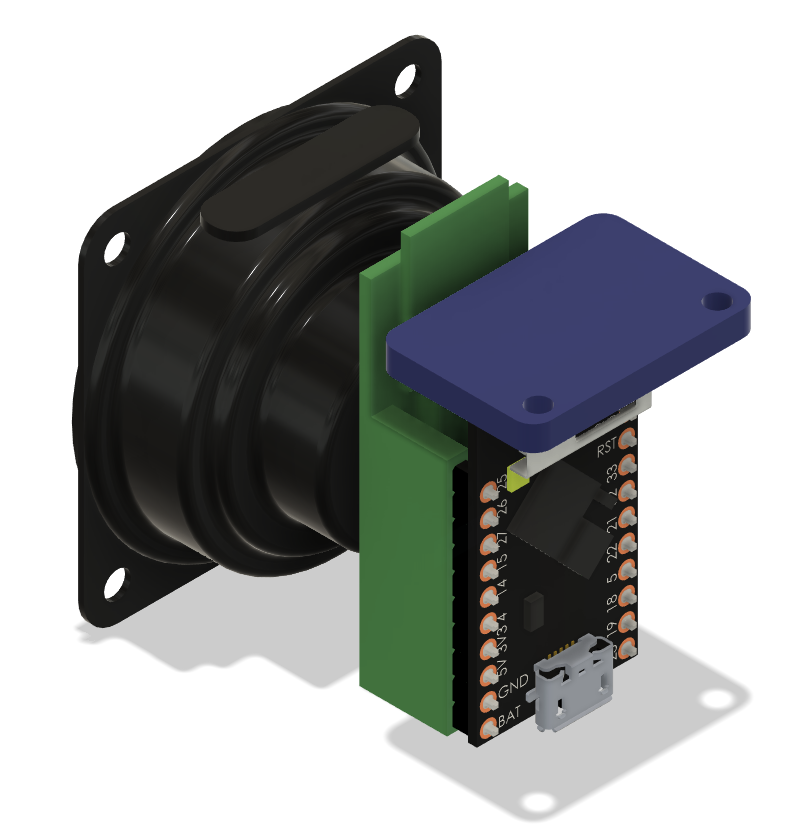
\includegraphics[width=0.4\textwidth,keepaspectratio, angle=0]{./figures/hardware.png}
            \caption{Hardware Locations within the CAD}
        \label{fig:hardware}
    \end{figure}

The hardware was arranged in a format that would allow for wiring, assembly and to take up the most minimal amount of space possible. This would be to satisfy the clients request of a minimal form factor

    \begin{figure}[ht!]
        \centering % Center tables
            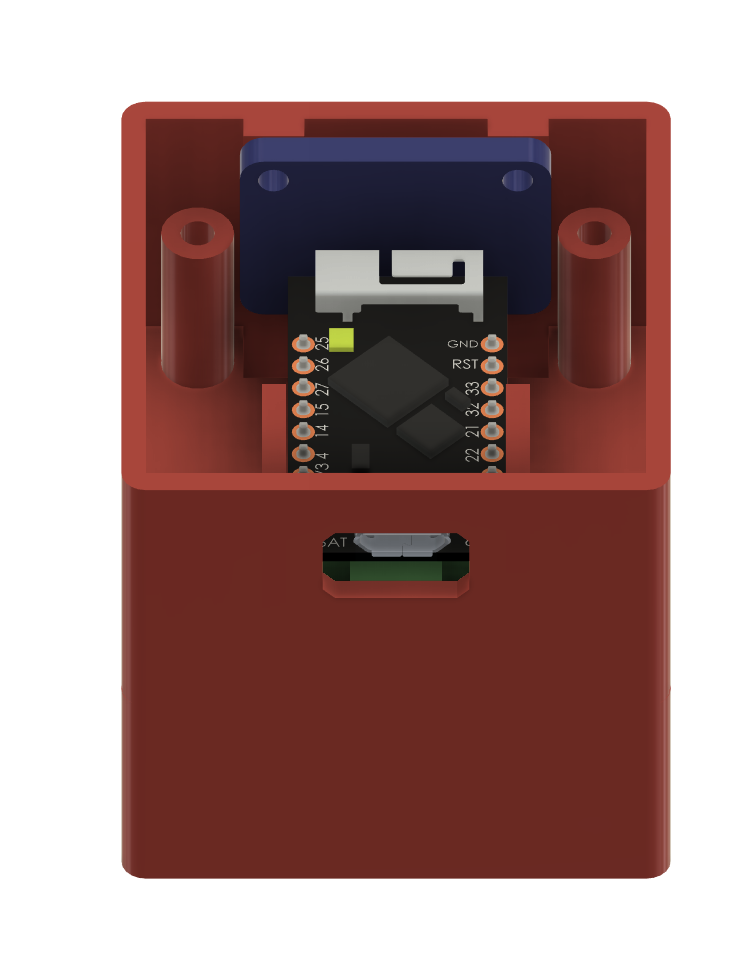
\includegraphics[width=0.4\textwidth,keepaspectratio, angle=0]{./figures/interior.png}
            \caption{Mid and Front casing arrangement}
            
            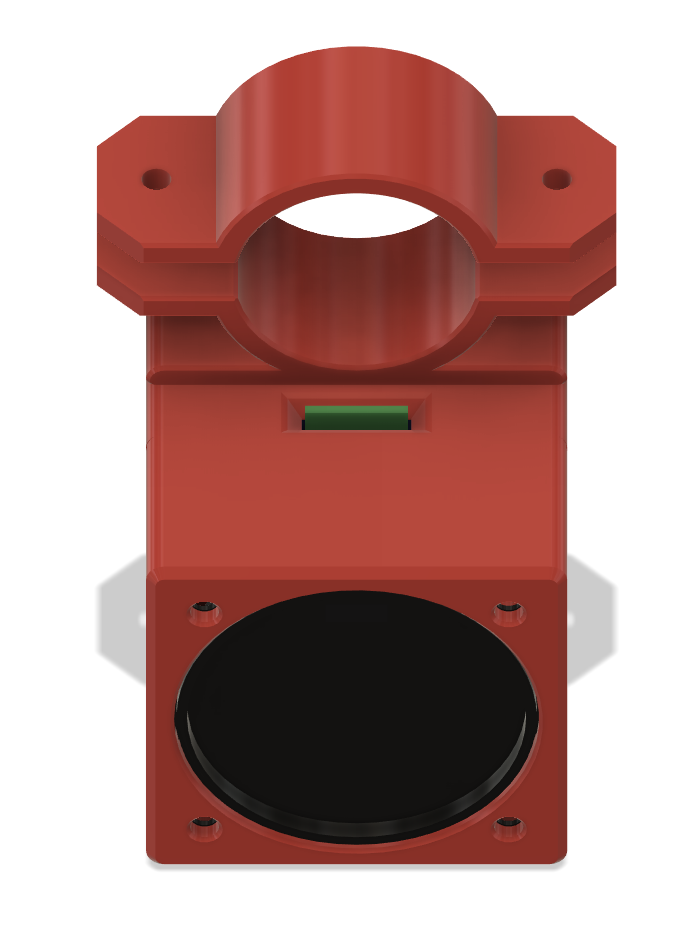
\includegraphics[width=0.4\textwidth,keepaspectratio, angle=0]{./figures/final-cad.png}
            \caption{Final CAD for prototype 1}
        \label{fig:interior}
    \end{figure}

The design uses spacers, as well as an front/end casing design that allows the mid housing to be used for secure attachment of all the pieces together. The spacers allow for the components inside to be held securely, and for minimal fasteners to be needed, aiding the assembly process.



Tolerances had to be calculated carefully due to our use of a Fused Deposition Modeling (FDM) printer, to ensure the end different parts would interface with eachother correctly.

\paragraph{3D Printing}

Upon finishing the CAD, the first prototype was printed using a Voron Design 0.1 FDM 3D Printer, using ABS plastic. It is a less common thermoplastic used in printing, but allows for good heat resistance beyond the needs of our small micro controllers, as well as excellent resistant to shock and deformation, allowing for a resistant prototype that can be correctly tested. The open source SuperSlicer was used to generate the gcode that was printed.

\paragraph{Assembly}

Assembly was simple as it was designed with it in mind, requiring the speaker to be connected using ferrules and the terminal connector on the audio shield, prior to the TinyPICO being placed onto the headers.

Wiring was completed with 26AWG silicone wire, which allowed for great flexibility and tight wiring paths.

    \begin{figure}[ht!]
        \centering % Center tables
            \includegraphics[width=0.4\textwidth,keepaspectratio, angle=90]{./figures/wiring.jpg}
            \caption{Internal wiring}
        \label{fig:wiring}
    \end{figure}
    
        \begin{figure}[ht!]
        \centering % Center tables
            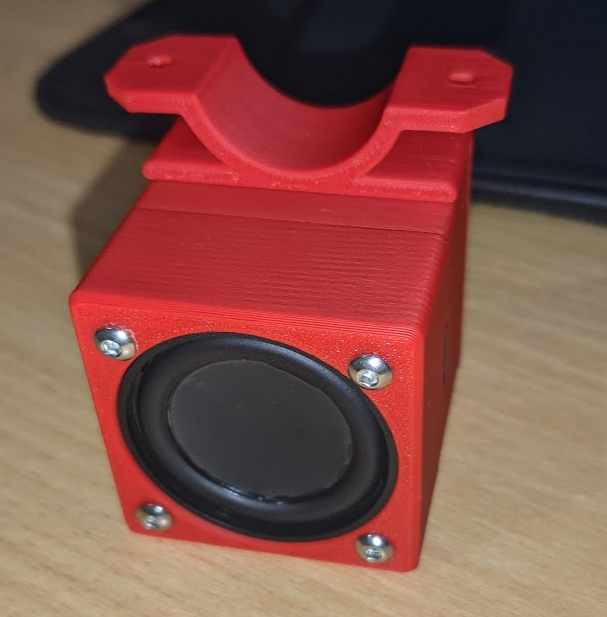
\includegraphics[width=0.4\textwidth,keepaspectratio, angle=0]{./figures/final-assembly.png}
            \caption{Final assembly}
        \label{fig:assembly}
    \end{figure}

\section{Future Work}
\label{subsec:future_work}

For this section, we will list all the work that we plan to implement in the very near future to advance our project and meet our schedule. For each item of work we list, we will detail what the work will entail and how it benefits the overall progress of the project.

\paragraph{Integrate communication system with walking detection system}

This work will provide the basis for the reminder system that needs to be developed that will allow us to play audio to the patient when they begin walking without their walking aid. The combination of this code should be fairly simple to implement and will allow us to replace the current code to flash the LED of the TinyPICO with code that will send a message to the walking aid to check if it is moving also. If it is not moving, then we can call code to play the reminder audio.

\paragraph{Develop BLE distance solution for walking detection}

For comparison against our already developed step-counting walking detection system, we want to develop a working solution for detecting walking with the use of BLE distance monitoring using its signal strength. This will allow us to receive real world analysis of each solution and be able to finalise on which system to use based on which is most suitable to our project.

\paragraph{Implement the reminder system}

We need to begin the development of code for the reminder system to allow for audio files to be played which will remind the patient to take their walking aid with them. Once the code for this has been developed, it can easily replace the reminder simulation we currently have implemented that flashes the LED of the TinyPICO device.

\paragraph{Develop walking aid movement detection system}

To identify whether the walking aid is moving with the patient and whether we need to play reminder audio or not, we need to create an Arduino sketch for the walking aid system itself is moving. The implementation for this should be fairly simple also, as we will use a similar system to our already developed single tap detection step-counter system on our wearable device. Each time the patient places the walking aid down on the floor for support, we will be able to detect a tap through the accelerometer and in turn be able to conclude that the walking aid is moving.

\paragraph{Refine 3D Model}

Upon assembly of the initial prototype, some issues were identified. More clearance will be required to make the SD Card more easily removable, as well as some internal structure/spacer will be required to support the TinyPICO from above, as the horizontal supports were not sufficient for this. 

Beyond this, the wearable device will also need to be designed, but we anticipate this to be much easier and simpler than the complex multi-part design for the walking aid.

\paragraph{Begin development of Milestone 3 document}

We aim to be able to hand over our project to the client with a fully documented user manual, and to do this it is necessary for us to complete our Milestone 3 to a good standard. It is imperative to the client that we begin development of this document as early as possible to ensure that all details are covered within the document and that final testing can take place with a high level of scrutiny.

}


\clearpage
\printbibliography

\end{document}
